\chapter{Websocket}
\label{chap:websocket}
\nocite{html5}
Nel capitolo \ref{chap:scelta} abbiamo parlato di come e con quali tecnologie sono state implementate le API REST di proximity system.  
Queste API danno la possibilità a chiunque di implementare un proprio client per qualsiasi dispositivo. 
Il problema di questi servizi è che che sono di tipo pull, ovvero dev'essere il client a chiedere informazioni al server. 
Il server non può inviare i dati aggiornati appena sono disponibili,
ma soltanto quando un client li richiede.
In questo capitolo andremo a vedere come risolvere questo problema il metodo di comunicazione più potente introdotto con la specifica HTML5: le WebSocket.
Queste non sono altro che un canale di comunicazione full-duplex operante su una singola socket che permette di migliorare drasticamente sia la quantità di traffico che la latenza di tutte le applicazione web basate sulla visualizzazione di dati in tempo reale e sugli eventi.
  
\section{Panoramica della applicazione real-time e HTTP}
\label{sec:real-time}
Prima di andare nel dettaglio nella specifica WebSocket, vediamo quali sono e come funzionano i principali "hack" utilizzati per simulare un'applicazione real-time con il protocollo HTTP.

Nei tradizionali siti web quando un server HTTP riceve una richiesta, il server genera la pagina richiesta personalizzata per il client la inoltra e il client che poi fa il render della risposta e la visualizza a video.
Esistono molti casi, come la disponibilità di biglietti per un evento, dati azionari etc. in cui i dati inviati dal server potrebbero già essere deprecati nel momento in cui il client fa il render della pagina. 
Per avere i dati aggiornati è necessario aggiornare i dati continuamente, ad esempio manualmente, anche se ovviamente non rappresenta una soluzione ottimale.

Comet\index{Comet} è un modello per le web application nel quale una particolare gestione 
delle richieste HTTP permette al web server di inviare notifiche push al browser, senza che il browser faccia una richiesta specifica.
Esistono diverse tecniche che permettono di implementare questo modello basato sugli eventi. 

La più diffusa tra le tecniche comet è il polling, che consiste nell'invio di richieste HTTP a intervalli regolari con una risposta immediata da parte del server. 
Questa tecnica è efficiente nei casi in cui si conosce a prescindere ogni quanto tempo i dati verranno aggiornati dal server.
Come è facile immaginare non è sempre facile prevedere con quale cadenza i dati verranno aggiornati, causando un numero elevato di richieste non necessarie.
Quello che ne deriva è l'apertura e la chiusura di un alto numero di connessioni e quindi l'utilizzo di risorse non strettamente necessarie.

Una possibile soluzione è l'implementazione del long-polling, dove il client invia una richiesta al server che risponderà soltanto se i dati sono stati aggiornati e farà scadere la richiesta altrimenti. È importante far notare che se il numero di aggiornamenti è alto, non si hanno vantaggi rispetto al polling tradizionale.
\begin{figure}[htpb!]
  \centering
  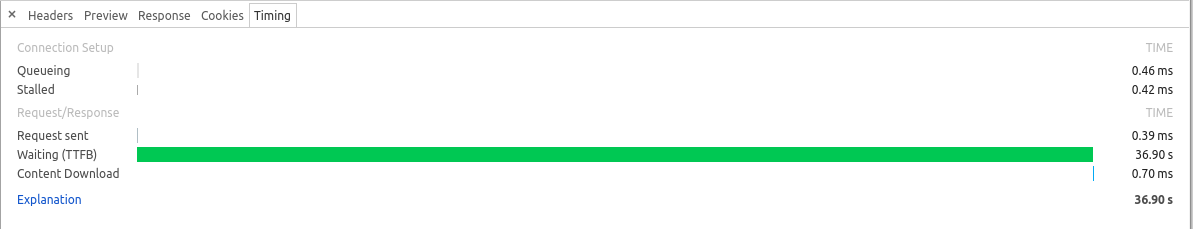
\includegraphics[width=1\textwidth]{timing}
  \caption{Esempio di long-polling}
  \label{fig:timing}
\end{figure}
Quello in Figura \ref{fig:timing} è un esempio di long-polling in azione preso da messenger. 

Un'altra tecnica, che prende il nome di streaming, consiste in una connessione completa tra client e server, in cui il server mantiene la connessione aperta con un aggiornamento costante delle informazioni per un tempo indeterminato, per poi aggiornare la risposta con l'arrivo di nuovi dati, sempre mantenendo aperta la connessione.

In questo modo la connessione rimane aperta per i messaggi seguenti.
Il problema è dato dal fatto che lo streaming è incapsulato in una richiesta HTTP e in quanto tale un eventuale firewall o proxy nel mezzo potrebbero interferire bufferizzando la risposta.
Per questo motivo molti sistemi passano automaticamente al long-polling se rilevano la presenza di qualche proxy.
Una possibile soluzione alternativa è quella di utilizzare connessioni TLS per impedire il buffering della risposta,
ma in questo caso bisogna prendere in considerazione utilizzo di
maggiori risorse da parte del server.

Tutte le tecniche sopra descritte hanno in comune due problemi:
\begin{itemize}
\item prevedono l'utilizzo dell'header HTTP
\item prevedono l'invio di messaggi solo dal server al client
\end{itemize}
Il primo problema consiste nel fatto che l'header HTTP contiene molte informazioni inutili al fine della comunicazione stessa, occupando banda e aumentando la latenza della connessione.

Il secondo consiste nel fatto in cui se l'utente ha la necessita di inviare dati al server, 
dovrà instaurare una nuova connessione per poterlo fare.
Ciò comporta tutta una serie di problematiche per mantenere i dati
sincronizzati tra tutte le connessione.

In altre parole, il protocollo HTTP 1.1 è un protocollo pull e non push.
In quanto tale, realizzare una webapp con il modello publish/subscribe attraverso comunicazioni HTTP half-duplex è più complicato di quanto sembri, sopratutto per soluzioni scalabili.

\section{Introduzione alle WebSocket}
Ian Hickson, uno dei principali responsabili della specifica HTML5, inizialmente definì le WebSocket nella sezione specifica dedicata ai metodi di comunicazione con il nome di "TCPConnection".
Questa specifica si è evoluta poi a tal punto da far definire le WebSocket in una specifica indipendente come la geolocalizzazione, i Web Worker etc. per mantenere la discussione focalizzata.

Il protocollo WebSocket viene descritto nel RFC 6455\cite{RFC6455} ed è diviso in due parti: una che descrive l'handshake e una per il trasferimento dei dati.

Una volta che il client e il server hanno completato l'handshake, se è andato a buon fine, allora i due possono iniziare a comunicare.
Quello che si crea è un canale di comunicazione full-duplex dove sia il client che il server, indipendentemente l'uno dall'altro, possono inviare dei dati.

Dopo l'handshake, i dati che vengono scambiati prendono il nome di "messaggi". 
A livello fisico, un messaggio è composto da uno o più frame.
Quindi un messaggio WebSocket non corrisponde necessariamente ad un particolare frame, in quanto il messaggio può essere frammentato e poi ricomposto da qualsiasi intermediario tra le due parti.

Un frame ha associato un determinato tipo. 
Ogni frame dello stesso messaggio contiene lo stesso tipo di dati.
Possiamo identificare dei dati di tipo testo(UTF-8), dati binari e frame di controllo.
La versione corrente del protocollo definisce sei tipi di frame e ne lascia altri dieci per future implementazioni.
\subsection{L'handshake WebSocket}
\label{sec:handshake}
L'handshake è stato progettato per essere compatibile con i server basati sul protocollo HTTP, in modo tale che una singola porta possa essere utilizzata sia dai client che vogliono comunicare con il WebServer sia dai client WebSocket.
Per questo motivo l'handshake è una richiesta di HTTP upgrade.
\begin{lstlisting}[caption={client handshake}, style=javaScriptCode]
	GET /chat HTTP/1.1
	Host: server.example.com
	Upgrade: websocket
	Connection: Upgrade
	Sec-WebSocket-Key: dGhlIHNhbXBsZSBub25jZQ==
	Origin: http://example.com
	Sec-WebSocket-Protocol: chat, superchat
	Sec-WebSocket-Version: 13
\end{lstlisting} 

Come stabilito nel RFC 2616, i campi dell'header possono essere inviati in qualsiasi ordine.  
Il metodo GET viene utilizzato sia per identificare la WebSocket corretta, sia per far in modo che domini multipli possano essere serviti da un singolo indirizzo IP e per permettere la gestione di più WebSocket in un singolo server.

Il client include nell'header il nome dell'host del server così come descritto in RFC2616\cite{RFC2616}, in modo tale che sia il client che il server
possano verificare che l'host in uso sia quello corretto.

Campi dell'header addizionali possono essere aggiunti  per selezionare
delle opzioni del protocollo WebSocket.
Le opzioni tipiche che vengono utilizzate sono:
\begin{itemize}
\item Sec-WebSocket-Protocol: lista dei sotto protocolli disponibili nel client;
\item Sec-WebSocket-Extension: lista delle estensioni disponibili nel client;
\item Origin: per la gestione del CORS.
\end{itemize}

Il campo \emph{Origin} vieni utilizzato come contromisura per 
l'utilizzo non autorizzato del server WebSocket da script eseguiti nel browser.
Se il server non vuole accettare una connessione da una determinata origine, 
può scegliere di rifiutare la connessione inviando un codice di errore HTTP appropriato.
Questo campo ha senso solo per i client che sono browser, in quanto tutti gli altri possono modificarlo a loro piacimento.

Adesso, il server deve dimostrare al client che ha ricevuto un messaggio di handshake e deve stare attento a non accettare richieste che non siano per le WebSocket.
In modo tale da prevenire eventuali attacchi generati con un XMLHttpRequest o l'invio di dati da un form.

Per dimostrare che ha ricevuto l'handshake corretto, il server deve mettere insieme due dati e metterli insieme per generare una risposta.
Il primo dato viene preso dal campo \emph{Sec-WebSocket-Key}.
il secondo è la stringa che rappresenta il GUID(Globally Unique Identifier RFC4122\cite{RFC4122}) "258EAFA5-E914-47DA-95CA-C5AB0DC85B11".
Ad esempio, se prendiamo i dati dal handshake precedente, 
il server deve concatenare il GUID e il \emph{Sec-WebSocket-Key} ottenendo la stringa "dGhlIHNhbXBsZSBub25jZQ==258EAFA5-E914-47DA-95CA-C5AB0DC85B11".
Poi il server deve prendere l'hash SHA-1 di questa stringa, ovvero 
0xb3 0x7a 0x4f 0x2c 0xc0 0x62 0x4f 0x16 0x90 0xf6 0x46 0x06 0xcf 0x38 0x59 0x45 0xb2 0xbe 0xc4 0xea.
Questo valore deve essere poi codificato in base64, 
ottenendo "s3pPLMBiTxaQ9kYGzzhZRbK+xOo=".
Questo valore dovrà essere inserito nell'header nel campo Sec-WebSocket-Accept".

L'handshake del server è molto più semplice rispetto a quello del client.

\begin{lstlisting}[caption={server handshake}, style=javaScriptCode]
	HTTP/1.1 101 Switching Protocols
	Upgrade: websocket
	Connection: Upgrade
	Sec-WebSocket-Accept: s3pPLMBiTxaQ9kYGzzhZRbK+xOo=
\end{lstlisting} 
\label{sec:serv_handshake}

Se il valore di Sec-WebSocket-Accept non è quello aspettato, se manca qualche header, o se lo stato HTTP è diverso da 101, la connessione non verrà stabilita e i frame WebSocket non verranno inviati.
L'header può anche includere i campi delle opzioni e settera eventuale cookie.
 
\subsection{L'interfaccia}
Utilizzare le WebSocket in un'applicazione JavaScript è molto semplice.
Per la connessione con l'host remoto è sufficiente creare una nuova istanza WebSocket, fornendo al nuovo oggetto l'URL con il quale si desidera aprire la connessione.
I prefissi \texttt{ws://} e \texttt{wss://} indicano rispettivamente una connessione WebSocket e una connessione WebSocket sicura.
La connessione WebSocket è stabilita passando dal protocollo HTTP a quello WebSocket, durante l'handshake iniziale tra client e server, attraverso la stessa connessione TCP/IP. Dopo aver stabilito la connessione i frame di dati WebSocket possono essere inviati e ricevuti in modalità full-duplex.
La connessione stessa è esposta tramite l'evento \texttt{message} e il metodo \texttt{send} definiti nell'interfaccia WebSocket.
Scrivendo il codice è possibile utilizzare dei \emph{listener} asincroni per gestire ogni fase del ciclo di connesione.
\begin{lstlisting}[caption={interfaccia WebSocket}, style=javaScriptCode]
url = "ws://example.com/echo";
socket = new WebSocket(url);
socket.onopen = function() {
	console.log("WebSocket aperta");
	socket.send("Grazie per aver accettato questa WebSocket");
}
socket.onmessage = function(e) {
	console.log(e.data);
}	
socket.onclose = function(e) {
	console.log("connessione chiusa");
}
\end{lstlisting} 
\label{sec:interfaccia_websocket}
\subsection{Aumento delle prestazioni}
Le WebSocket HTML offrono vantaggi tali da spingere Ian Hickson (Google) a dichiarare: \\
\textit{"Reducing kilobytes of data to 2 bytes is more than "a little more byte efficient", 
and reducing latency from 150ms (TCP round trip to set up the 
connection plus a packet for the message) to 50ms (just the packet for the 
message) is far more than marginal. 
In fact, these two factors alone are enough to make WebSocket seriously interesting to Google."}\footnote{\url{www.ietf.org/mail-archive/web/hybi/current/msg00784.html}}
  
Per illustrare quanto possono essere efficienti le WebSocket,
andremo a confrontare il traffico e la latenza di un'applicazione web prima implementata tramite polling e poi tramite WebSocket.

Dato che il miglioramento delle performance in Proximity System è minimo, 
prenderemo in considerazione un'ipotetica applicazione che visualizza dati in tempo reale i dati di una macchina da corsa: velocità; giri del motore; tempo del giro, posizione, km percorsi.
Supponiamo che le 2 nostre applicazioni, quella basata sul polling e qualle basata sulle WebSocket, ricevano i dati tramite il seguente JSON:
\begin{lstlisting}[caption={JSON dati macchina}, style=javaScriptCode]
{
	"lap_time": "35.256", 
	"speed": "124",
	"gear": "4",
	"RPM": "15600",
	"mileage": "12563.02"
}
\end{lstlisting} 

In questo caso la quantità di dati che il server invia al client è pari al numero di caratteri presenti nel JSON, escludendo gli spazi, le tabulazioni e i ritorni a capo che si possono omettere contiamo 81 caratteri e quindi 81 byte di dati.
Il problema è che oltre agli 81 byte dei dati effettivi, ogni richiesta XMLHttpRequest deve considerare sia l'header inviato dal client che quello inviato dal server in risposta.
Giusto per far un esempio, osserviamo i due header di una richiesta fatta utilizzando ProximitySystem
\begin{lstlisting}[caption={header client}, style=javaScriptCode]
GET /api/v2.0/gpio HTTP/1.1\r\n
Host: localhost:8000
Connection: keep-alive
Cache-Control: max-age=0
Accept: application/json, text/plain, */*
If-Non-Match: If-None-Match: W/"4dc-Uz68k8B/IopHdTlOHcquQA"
User-Agent: Mozilla/5.0 (X11; Linux x86_64) AppleWebKit/537.36 (KHTML, like Gecko) 
				Chrome/52.0.2743.116 Safari/537.36
Authorization: Basic YWRtaW46MTIzNDU2
DNT: 1
Referer: http://localhost:8000/
Accept-Encoding: gzip, deflate, sdhc
Accept-Language: it-IT,it;q=0.8,en-US;q=0.6,en;q=0.4
\end{lstlisting}
Solo nell'header di richiesta ci sono 484 caratteri
\begin{lstlisting}[caption={header server}, style=javaScriptCode]
HTTP/1.1 200 OK
X-Powered-By: Express
Content-Type: application/json; charset=utf-8
Content-Length: 1246
Etag: W/"4de-K40aEhIMswWt/3FPFcGKCQ"
Date: Mon, 29 Aug 2016 15:05:16 GMT
Connection: keep-alive

\end{lstlisting} 
Aggiungendo i 210 della risposta otteniamo 694 byte di dati non necessari per ogni richiesta. 
È vero che queso è solo un esempio, e ci saranno situazioni con meni dati nell'header, ma è bene sapere che in alcuni casi le informazioni nell'header possono arrivare vino a 2000 byte.
Andando a ricapitolare possiamo vedere come il rapporto tra dati inutili(694 byte) e dati utili(81 byte) sia di  circa 8:1, un gran spreco di dati.
Vediamo cosa accadrebbe distribuendo questa applicazione ad un ampio numero di utenti. 
ipotizziamo tre scenari di utilizzo:
\begin{enumerate}
\item 1.000 client che eseguono il polling ogni secondo.
il traffico equivale a: 694 x 1.000 = 694.000 byte = 5.552.000 bit al secondo = 5,2 Mbps;
\item 10.000 client che eseguono il polling ogni secondo.
il traffico equivale a: 694 x 10.000 = 6.940.000 byte = 55.520.000 bit al secondo = 52 Mbps;
\item 100.000 client che eseguono il polling ogni secondo.
il traffico equivale a: 694 x 100.000 = 69.400.000 byte = 555.200.000 bit al secondo = 529 Mbps.
\end{enumerate}
Adesso che abbiamo visto la quantità di banda che si spreca utilizzando il polling, 
andiamo ad analizzare come si comporta la stessa applicazione con l'utilizzo delle WebSocket.
\begin{figure}[htpb!]
  \centering
  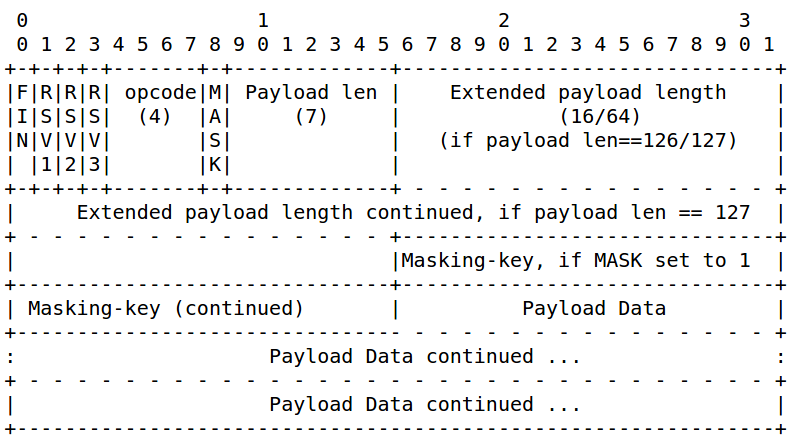
\includegraphics[width=1\textwidth]{frame}
  \caption{Frame WebSocket}
  \label{fig:frame}
\end{figure}
Osservando il frame si può evincere che le informazioni non necessarie possono variare da un minimo di 2 byte ad un massimo di 16 byte.
Ecco lo scenario del traffico prendendo in considerazione il caso peggiore:
\begin{enumerate}
\item 1.000 client che ricevono un messaggio al secondo.
il traffico equivale a: 16 x 1.000 = 16.000 byte = 128.000 bit al secondo = 0,12 Mbps;
\item 10.000 client che ricevono un messaggio al secondo.
il traffico equivale a: 16 x 10.000 = 160.000 byte = 1.280.000 bit al secondo = 1,22 Mbps;
\item 100.000  client che ricevono un messaggio al secondo.
il traffico equivale a: 16 x 100.000 = 1.600.000 byte = 12.800.000 bit al secondo = 12,20 Mbps.
\end{enumerate}
\begin{figure}[htpb!]
  \centering
  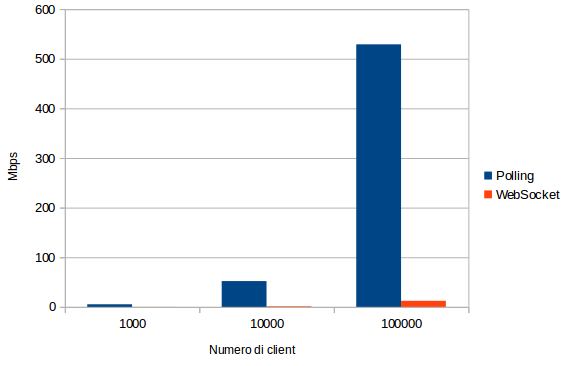
\includegraphics[width=0.8\textwidth]{dati_non_necessari}
  \caption{Traffico dati non necessario}
  \label{fig:traffico}
\end{figure}
Basta guardare la Figura \ref{fig:traffico} per rendersi conto dell'inutile mole di dati che viene generata se si realizza un'applicazione real-time con il polling.

Per quanto riguarda la latenza, l'aumento delle performance è illustrate in Figura \ref{fig:latenza}.
Se ipotizziamo che un pacchetto per arrivare dal browser al server impieghi 50 ms, l'applicazione con il polling genera molta latenza in più rispetto a quella implementata tramite WebSocket, 
perché per ogni risposta completa deve essere inviata una nuova richiesta.    
\begin{figure}[htpb!]
  \centering
  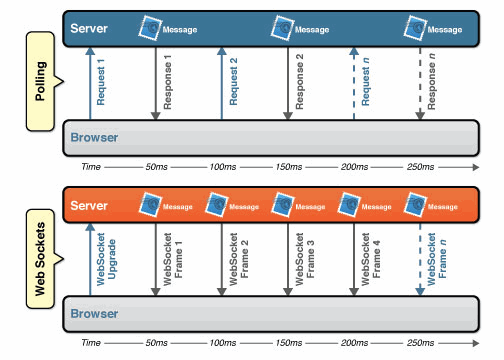
\includegraphics[width=0.8\textwidth]{latenza}
  \caption{Latenza}
  \label{fig:latenza}
\end{figure}
\subsection{Supporto dei browser}
La specifica WebSocket ormai ha qualche anno, per la precisione, la versione standard definita nel RFC6455 è di dicembre 2011.
Nonostante ciò, le WebSocket sono supportate solo nei browser più recenti.
\begin{table}[htbp]
\begin{center}
\begin{tabular}{|l|l|l|l|l|l|}
\hline
Versione & Chrome & Firefox & Internet Explorer & Opera & Safari \\
\hline
76 & 6 & 4.0 & No & 11.00(disabilitato) & 5.0.1\\
\hline
7 & No & 6.0 & No & No & No \\
\hline
10 & 14 & 7.0 & HTML5 Labs & ? & ?\\
\hline
RFC 6455 & 16 & 11.0 & 10 & 12.10 & 6.0\\
\hline
\end{tabular}
\end{center}
\caption{Supporto dei browser}
\label{tab:browser}
\end{table}

\begin{table}[htbp]
\begin{center}
\begin{tabular}{|l|l|l|l|l|l|}
\hline
Versione & Android & Firefox Mob. & IE Mob. & Opera Mob. & Safari Mob.\\
\hline
76 & ? & ? & ? & ? & ?\\
\hline
7 & ? & ? & ? & ? & ? \\
\hline
10 & ? & 7.0 & ? & ? & ?\\
\hline
RFC 6455 & 16(Chrome) & 11.0 & ? & 12.10 & 6.0\\
\hline
\end{tabular}
\end{center}
\caption{Supporto dei browser Mobile}
\label{tab:mobile}
\end{table}
Nelle Tabelle \ref{tab:browser} e \ref{tab:mobile} è possibile vedere, rispettivamente per desktop e per mobile, il supporto dei vari browser per le diverse specifiche delle WebSocket.

Quando si crea una WebApp con le WebSocket è importante prendere in considerazione anche la possibilità che esse non siano supportate dal client e quindi implementare anche una soluzione alternativa, per l'appunto, nel caso non sia possibile utilizzare le WebSocket.
Esistono diversi framework che forniscono supporto completo sia per l'implementazione del client che del server che risolvono tutti i problemi di compatibilità che potrebbero presentarsi.
Tra i framework più popolari troviamo:
\begin{itemize}
\item Kaazing;
\item LightStreamer; 
\item Socket.io.
\end{itemize}
Nel paragrafo successivo vedremo in dettaglio come implementare sia il client ed il server di un'applicazione real-time con Socket.io

\section{Socket.io}
\label{sec:socket.io}
Socket.io permette di sviluppare applicazione client-server real-time, 
senza doversi preoccupare delle problematiche relative alle WebSocket.
Ad esempio, se un client non supporta le WebSocket, socket.io implementerà lo stesso servizio con il polling, il tutto in maniera trasparente al programmatore.

In questa sezione scriveremo il codice di una chat, lo stesso proposto nel sito di Socket.io ma utilizzando Angular nel client, 
per farne vedere sia l'utilizzo lato frontend che backend.

\subsection{Backend}
Le uniche dipendenze di cui ha bisogno il nostro backend sono: express e socket.io.
Il codice è molto semplice e non ha bisogno di particolari spiegazioni.
Il server è in ascolto sulla porta 3000 sia di connessioni HTTP sia WebSocket.
Se riceve una richiesta http risponderà con la WebApp in Angular,
altrimenti, gestirà la WebSocket.
\begin{lstlisting}[caption={backend chat socket.io}, style=javaScriptCode]
var express = require('express');

var app = express();
var http = require('http').Server(app);
var io = require('socket.io')(http);
var port = 3000;

app.use(express.static(__dirname + '/angular'));

io.on('connection', function(socket){
  console.log('a user connected');

  socket.on('disconnect', function(){
    console.log('user disconnected');
  });

  socket.on('chat message', function(msg){
    console.log('message: ' + msg);
    io.emit('chat message', msg);
  });
});

http.listen(port, function(){
  console.log("Server listening on port " + port);
});
\end{lstlisting} 
L'unica cosa che fa il server è inviare in broadcast a tutte le socket connesse i messaggi che riceve dalle singoli connessioni.
Se non avessimo utilizzato Socket.io avremmo dovuto implementare soluzioni alternative nel caso in cui le WebSocket non fossero disponibili nel client o 
l'handshake non andasse a buon fine, in questo caso, invece, è Socket.io che si occupa di gestire tutti i possibili problemi e fornire una soluzione equivalente, in maniera sempre trasparente al programmatore.
\subsection{Frontend}
Il frontend, molto semplicemente, invierà i messaggi scritti dall'utente tramite Socket.io al server e visualizzerà a video i messaggi ricevuti dal server, il tutto, real-time.
Per utilizzare Socket.io come se fosse un servizio di Angular, 
abbiamo installato il plugin \texttt{angular-socket-io}, disponibile tramite bower e inizializzato come segue.
\begin{lstlisting}[caption={service mySocket}, style=javaScriptCode]
angular.module('socketApp.services.socket',[])
.factory('mySocket', function(socketFactory) {
  var myIoSocket = io.connect();

    mySocket = socketFactory({
      ioSocket: myIoSocket
    });

  return mySocket;
});
\end{lstlisting} 
A livello di controller basta iniettare il servizio come dipendenza e si
possono utilizzare i listener e i metodi messi a disposizione da Socket.io.
Nel codice che segue semplicemente se arriva un nuovo messaggio viene aggiunto all'array di messaggi.
\begin{lstlisting}[caption={controller mySocket}, style=javaScriptCode]
angular.module('socketApp.controllers.home', [])
.controller('HomeCtrl',  function($scope, mySocket) {
  $scope.messages = [];
  $scope.message = "Scrivi qualcosa";

  mySocket.on('chat message', function(data) {
    $scope.messages.push({text: data});
  })

  $scope.send = function() {
    mySocket.emit('chat message', $scope.message);
    $scope.message = "";
  };
});
\end{lstlisting} 
Questo è tutto, il codice completo dell'esempio è disponibile sul mio GitHub\footnote{\url{https://github.com/save91/angular-chat-socket.io}}.



